\documentclass[../DoAn.tex]{subfiles}
\begin{document}

\section{Tổng quan triển khai và đánh giá}

Chương này trình bày quá trình triển khai hệ thống JobBridge AI và đánh giá thực nghiệm trên môi trường đã triển khai. Khác với Chương 3, nơi tập trung vào phân tích yêu cầu và thiết kế nghiệp vụ, chương này tập trung vào kết quả hiện thực hóa hệ thống, cách các chức năng được cung cấp cho người dùng, quy trình phát hành tự động và khả năng vận hành dưới tải.

Mục tiêu đánh giá thực nghiệm gồm ba nội dung chính. Thứ nhất, kiểm chứng hệ thống có thể được phát hành tự động từ mã nguồn đến môi trường production thông qua CI/CD và Argo CD. Thứ hai, kiểm chứng các chức năng người dùng chính đã được triển khai thành giao diện hoàn chỉnh. Thứ ba, đánh giá khả năng vận hành của hệ thống khi tải tăng, đặc biệt là khả năng giám sát và tự động mở rộng số lượng Pod thông qua Horizontal Pod Autoscaler.

\section{Kết quả hiện thực hóa hệ thống}
\label{sec:hien-thuc-hoa-he-thong}

Hệ thống được hiện thực theo mô hình web application. Phía giao diện sử dụng React và TypeScript; phía backend gồm các service viết bằng Go, kết hợp với MongoDB, Cloudinary và LLM API.

Các thành phần này được đóng gói bằng container, triển khai lên Azure Kubernetes Service và được quản lý bằng Helm chart.

Bảng \ref{tab:implemented-components} tổng hợp các thành phần chính đã được hiện thực trong phạm vi đồ án.

\begin{table}[H]
\centering
\caption{Thành phần hệ thống đã hiện thực}
\label{tab:implemented-components}
\begin{tabular}{|p{0.28\textwidth}|p{0.58\textwidth}|}
\hline
\textbf{Nhóm thành phần} & \textbf{Kết quả hiện thực} \\ \hline
Frontend & Giao diện cho khách truy cập, ứng viên, nhà tuyển dụng và quản trị viên. \\ \hline
Backend service & Gateway, Auth Service, Jobs Service và AI Service. \\ \hline
Cơ sở dữ liệu & MongoDB với các collection chính phục vụ người dùng, công ty, tin tuyển dụng và hồ sơ ứng tuyển. \\ \hline
Lưu trữ tệp & Cloudinary lưu avatar và CV; MongoDB lưu đường dẫn tệp và nội dung CV đã trích xuất. \\ \hline
AI & AI Interview Coach, AI Interview Quiz và đánh giá CV theo JD. \\ \hline
Triển khai & Docker image, Helm chart, AKS, ACR, Argo CD, Prometheus và Grafana. \\ \hline
\end{tabular}
\end{table}

Sản phẩm được triển khai trên tên miền công khai của hệ thống. Các chức năng đã triển khai bám sát 15 use case ở Chương 3, trong đó các màn hình chính được trình bày ở phần tiếp theo.

\section{Giao diện chức năng đã triển khai}
\label{sec:giao-dien-da-trien-khai}

\subsection{Giao diện xác thực người dùng}

Hình \ref{fig:ui-auth} minh họa hai màn hình xác thực cơ bản của hệ thống. Ở màn hình đăng ký, phần bên trái là biểu mẫu tạo tài khoản gồm họ tên, email, mật khẩu, điều khoản sử dụng và nút đăng ký; phần bên phải là khối nhận diện thương hiệu JobBridge AI, mô tả giá trị của hệ thống và thông điệp hỗ trợ người dùng khởi đầu sự nghiệp.

Ở màn hình đăng nhập, bố cục được đảo chiều để tạo sự khác biệt thị giác. Bên trái là phần giới thiệu thương hiệu và lời chào người dùng quay lại hệ thống; bên phải là biểu mẫu đăng nhập gồm email, mật khẩu, liên kết quên mật khẩu, nút đăng nhập và các lựa chọn đăng nhập bằng tài khoản mạng xã hội. Cách bố trí này giúp người dùng nhận diện rõ hành động chính trong từng màn hình.

\begin{figure}[H]
    \centering
    \makebox[\textwidth][c]{%
    \begin{subfigure}[b]{0.55\textwidth}
        \centering
        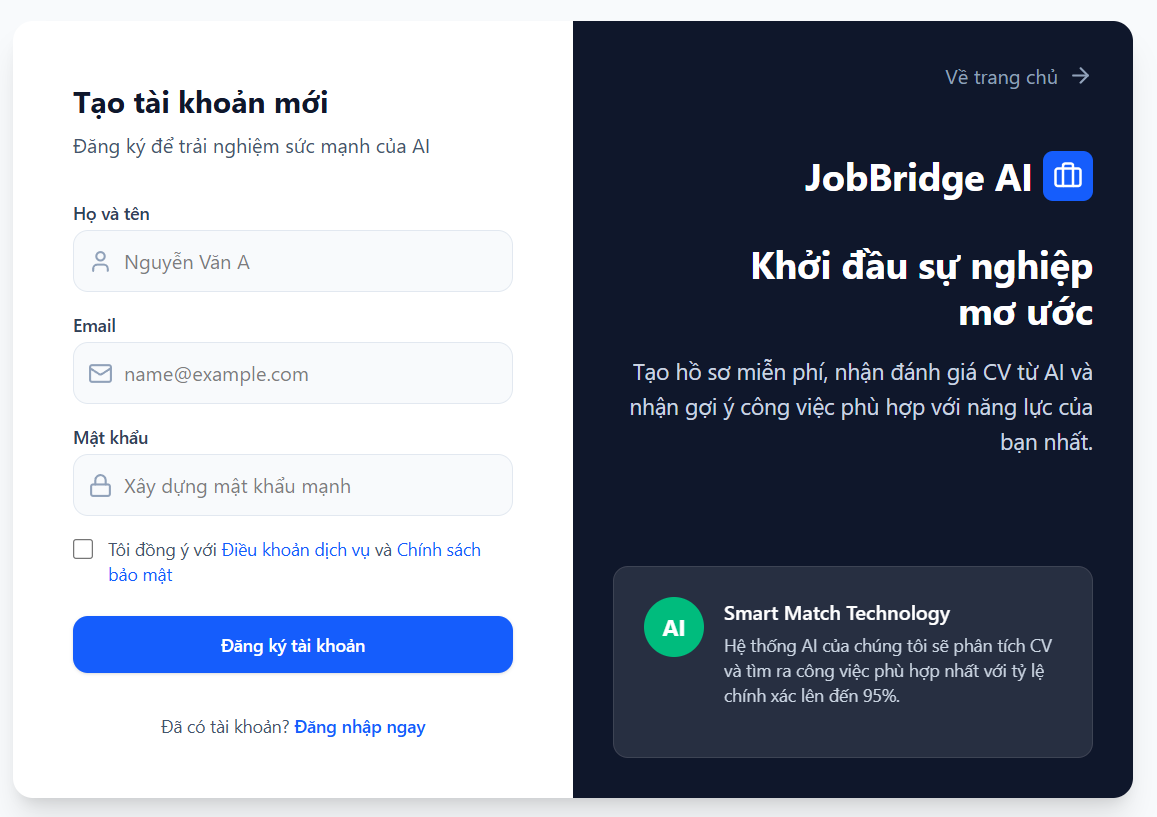
\includegraphics[width=\textwidth]{so-do-chuong-4/screens/màn hình đăng ký.png}
        \caption{Màn hình đăng ký}
    \end{subfigure}
    \hspace{0.03\textwidth}
    \begin{subfigure}[b]{0.55\textwidth}
        \centering
        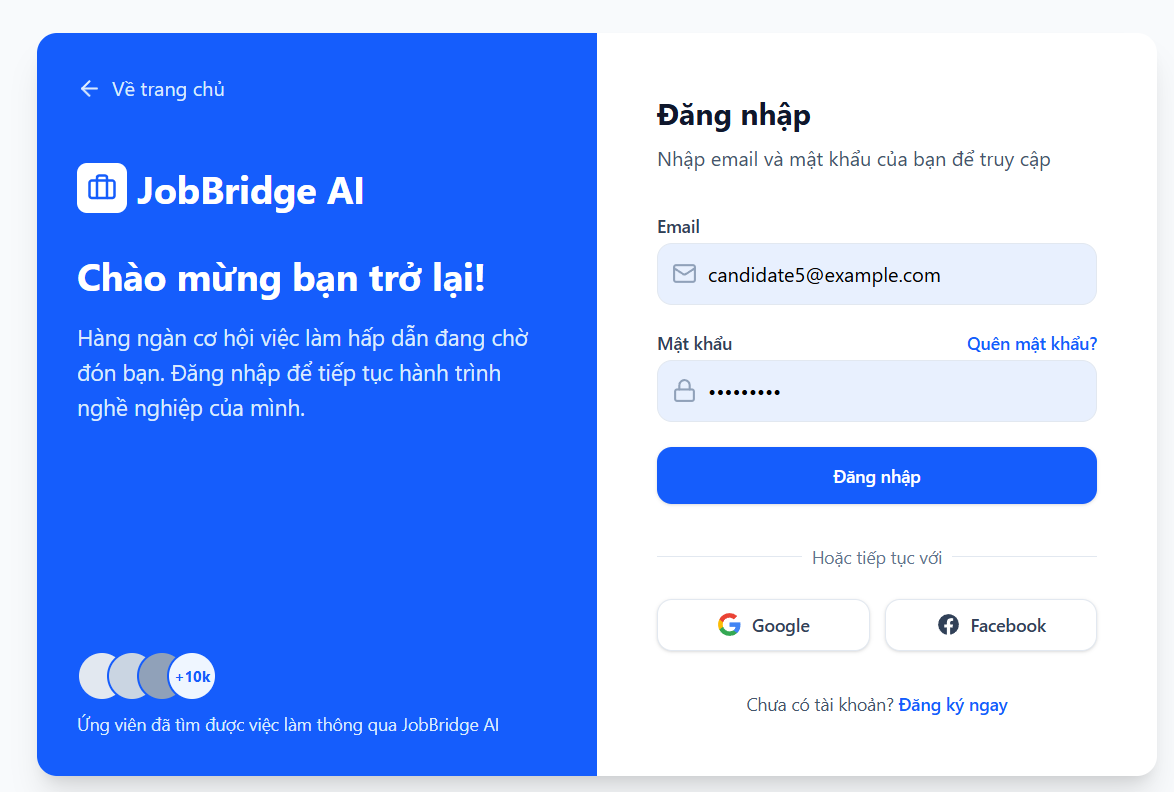
\includegraphics[width=\textwidth]{so-do-chuong-4/screens/man_hinh_dang_nhap.png}
        \caption{Màn hình đăng nhập}
    \end{subfigure}%
    }
    \caption{Giao diện xác thực người dùng}
    \label{fig:ui-auth}
\end{figure}

\subsection{Giao diện tìm kiếm việc làm}

Hình \ref{fig:ui-job-list} là giao diện danh sách việc làm dành cho ứng viên. Phía trên cùng là thanh điều hướng và khu vực tìm kiếm nhanh theo vị trí, kỹ năng hoặc công ty. Bên trái màn hình là bộ lọc theo mức lương và hình thức làm việc, giúp ứng viên thu hẹp danh sách kết quả mà không cần rời khỏi trang.

Khu vực bên phải là danh sách các tin tuyển dụng. Mỗi thẻ việc làm hiển thị tên vị trí, công ty, địa điểm, mức lương, hình thức làm việc, nhóm kỹ năng và ngày đăng. Cách trình bày dạng thẻ giúp người dùng so sánh nhanh nhiều vị trí trước khi mở chi tiết hoặc ứng tuyển.

\begin{figure}[H]
    \centering
    \makebox[\textwidth][c]{%
        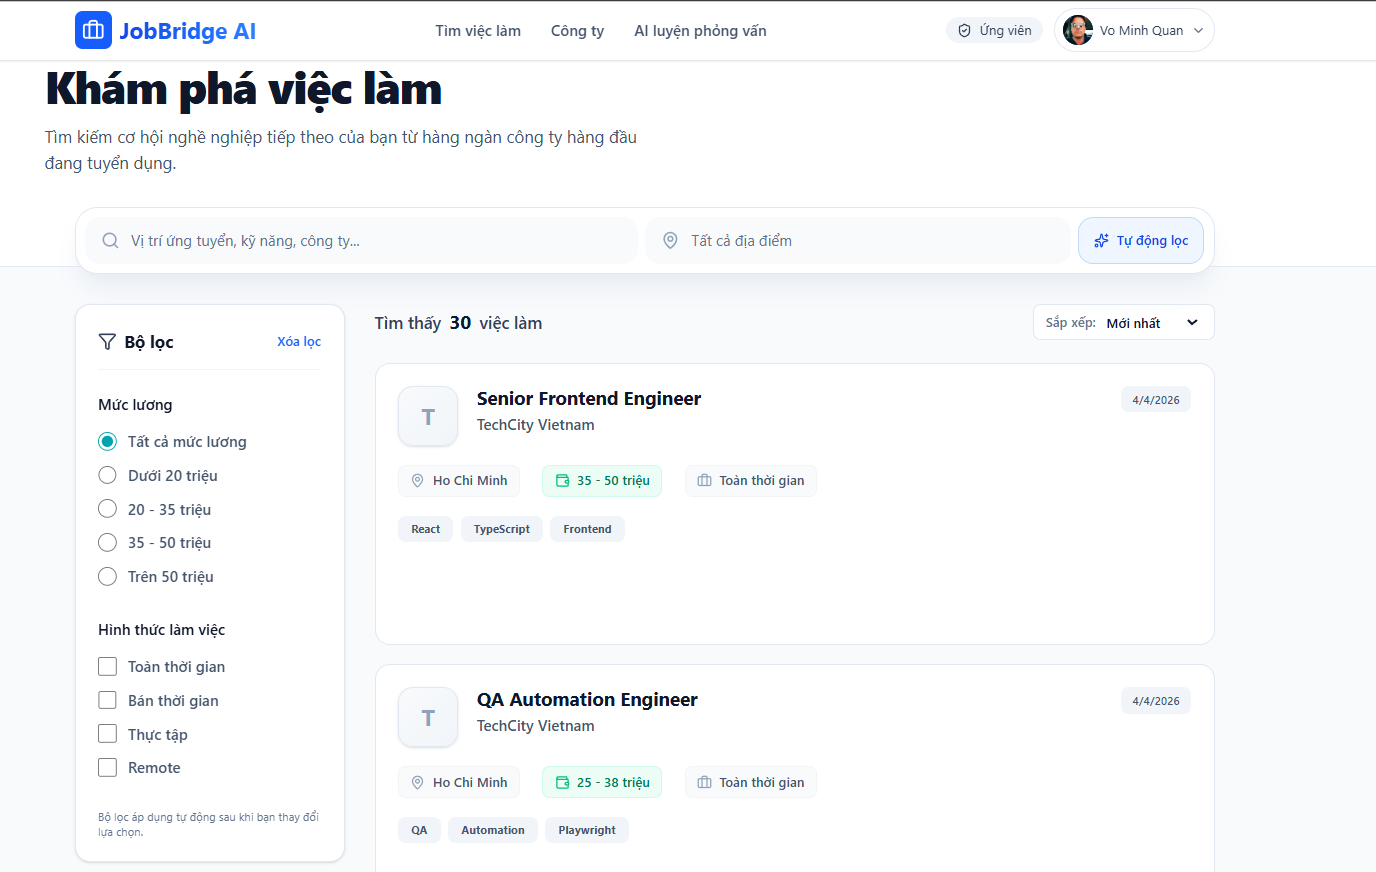
\includegraphics[width=1.15\textwidth]{so-do-chuong-4/screens/màn hình danh sách việc làm.png}%
    }
    \caption{Giao diện tìm kiếm và danh sách việc làm}
    \label{fig:ui-job-list}
\end{figure}

\subsection{Giao diện AI Interview Coach}

Hình \ref{fig:ui-ai-coach} thể hiện màn hình luyện phỏng vấn bằng AI dành cho ứng viên. Bên trái là cột ngữ cảnh, gồm danh sách job đã ứng tuyển, thông tin CV hiện tại và khu vực tạo quiz theo JD. Nhờ đó, ứng viên có thể kiểm soát dữ liệu đầu vào mà AI sử dụng trước khi bắt đầu luyện tập.

Bên phải là vùng hội thoại chính với AI Interview Coach. Khu vực này hiển thị các phản hồi của AI, ô nhập câu hỏi hoặc câu trả lời của ứng viên và nút gửi. Việc tách cột ngữ cảnh và cột hội thoại giúp người dùng vừa theo dõi vị trí đang luyện tập, vừa tập trung vào nội dung phỏng vấn.

\begin{figure}[H]
    \centering
    \makebox[\textwidth][c]{%
        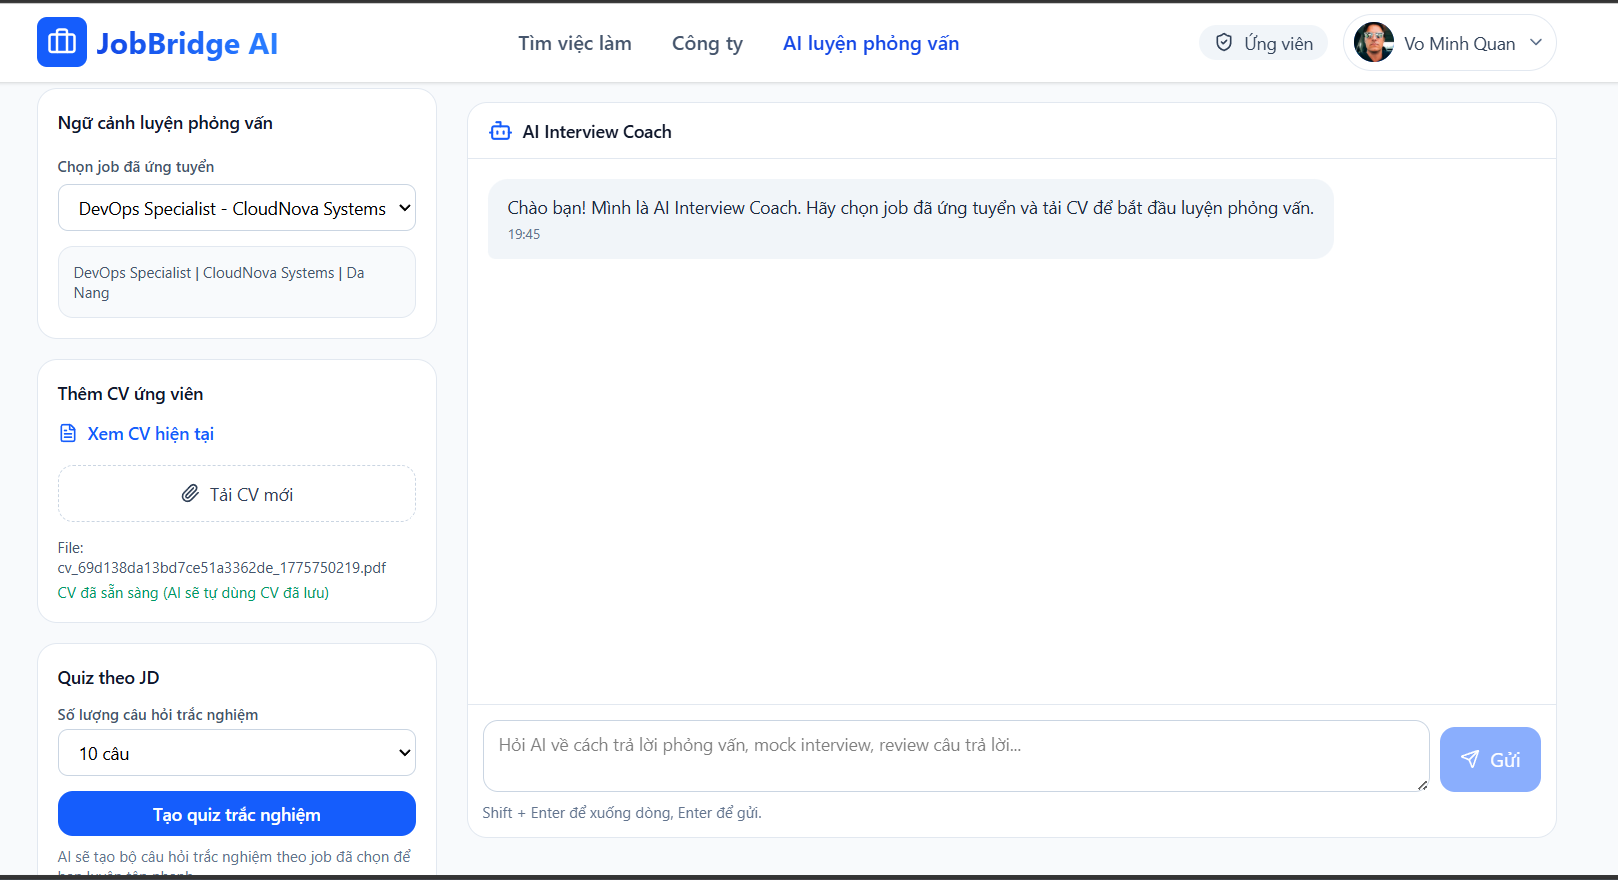
\includegraphics[width=1.15\textwidth]{so-do-chuong-4/screens/màn hình ai-coach.png}%
    }
    \caption{Giao diện AI Interview Coach}
    \label{fig:ui-ai-coach}
\end{figure}

\subsection{Giao diện quản lý tin tuyển dụng}

Hình \ref{fig:ui-hr-manage-jobs} minh họa màn hình quản lý tin tuyển dụng của nhà tuyển dụng. Bên trái là thanh điều hướng theo chức năng HR, giúp chuyển giữa các nhóm thao tác như quản lý công ty, quản lý job, danh sách ứng viên và đánh giá CV. Phần trung tâm là biểu mẫu tạo hoặc cập nhật tin tuyển dụng, gồm tiêu đề job, tên công ty, địa điểm, mức lương, loại hình làm việc, cấp độ kinh nghiệm và trạng thái tin.

Bên phải là danh sách job hiện có của nhà tuyển dụng. Khi chọn một job trong danh sách, thông tin chi tiết được đưa vào biểu mẫu ở giữa để chỉnh sửa. Cách bố trí này giúp nhà tuyển dụng vừa xem được toàn bộ danh sách vị trí đang đăng, vừa cập nhật nhanh từng tin tuyển dụng mà không phải chuyển trang nhiều lần.

\begin{figure}[H]
    \centering
    \makebox[\textwidth][c]{%
        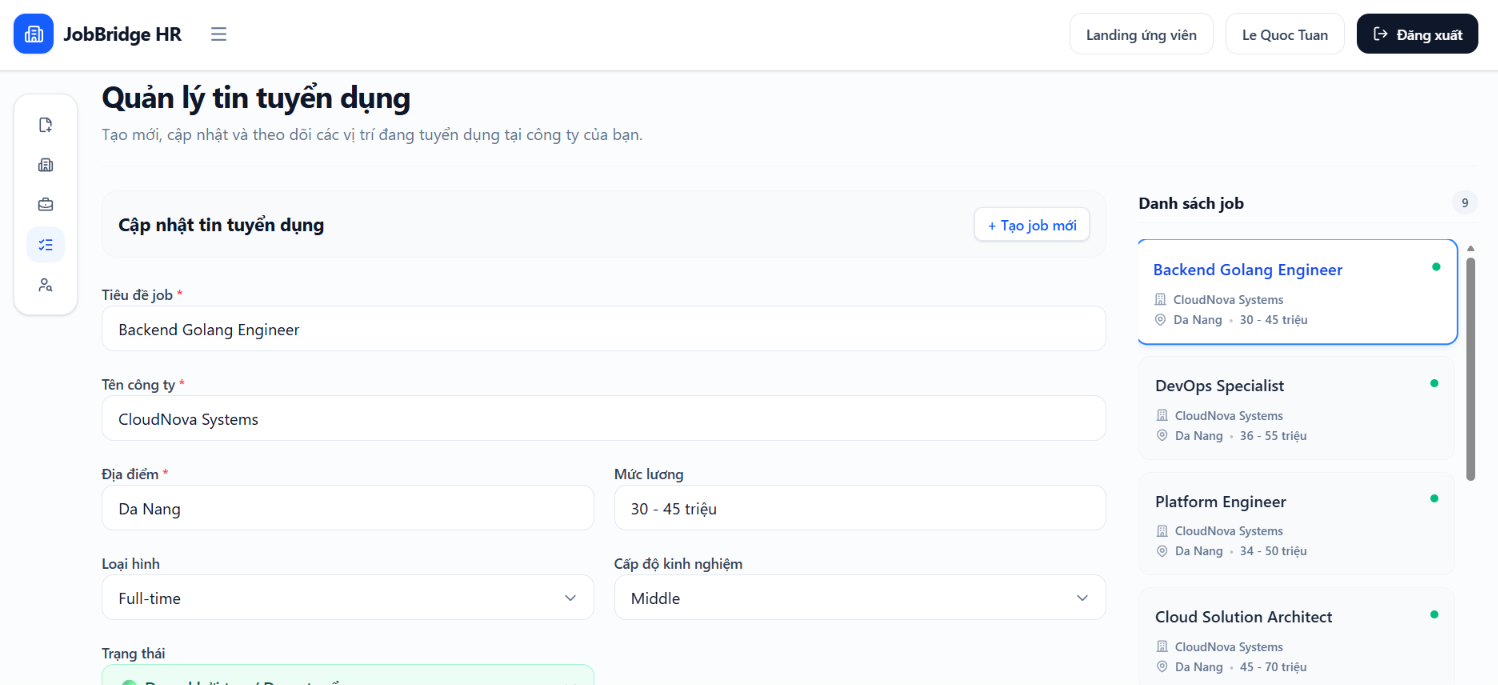
\includegraphics[width=1.15\textwidth]{so-do-chuong-4/screens/quản lý tin tuyển dụng.png}%
    }
    \caption{Giao diện quản lý tin tuyển dụng của nhà tuyển dụng}
    \label{fig:ui-hr-manage-jobs}
\end{figure}

\subsection{Giao diện AI đánh giá CV}

Hình \ref{fig:ui-hr-ai-evaluate} là màn hình hỗ trợ nhà tuyển dụng đánh giá CV bằng AI. Bên trái hiển thị thông tin ứng viên, vị trí ứng tuyển và trình xem PDF của CV gốc. Nhà tuyển dụng có thể mở CV để kiểm tra nội dung chi tiết trước khi đưa ra quyết định.

Bên phải là kết quả phân tích của AI, gồm điểm tương thích tổng thể, phần nhận xét, nhóm kỹ năng phù hợp, điểm mạnh và các điểm cần cải thiện. Thiết kế này không thay thế quyết định của nhà tuyển dụng, mà đóng vai trò công cụ hỗ trợ sàng lọc ban đầu và giúp việc đọc CV có định hướng hơn.

\begin{figure}[H]
    \centering
    \makebox[\textwidth][c]{%
        
\includegraphics[width=1.15\textwidth]{so-do-chuong-4/screens/màn hình AI đánh giá cv ứng viên.png}%
    }
    \caption{Giao diện AI đánh giá CV ứng viên}
    \label{fig:ui-hr-ai-evaluate}
\end{figure}

\subsection{Giao diện dashboard quản trị}

Hình \ref{fig:ui-admin} là dashboard dành cho quản trị viên. Bên trái là thanh điều hướng quản trị, gồm các mục Dashboard, Users và Companies. Phía dưới thanh điều hướng có khu vực System Health để thể hiện trạng thái tổng quan của API chính.

Khu vực bên phải là nội dung dashboard, gồm các thẻ thống kê tổng số người dùng, tổng số công ty và tổng số tin tuyển dụng. Góc phải phía trên hiển thị trạng thái hoạt động của hệ thống và thông tin tài khoản quản trị viên. Giao diện này phục vụ việc quan sát nhanh tình trạng nền tảng và đi đến các màn hình quản trị chi tiết khi cần.

\begin{figure}[H]
    \centering
    \makebox[\textwidth][c]{%
        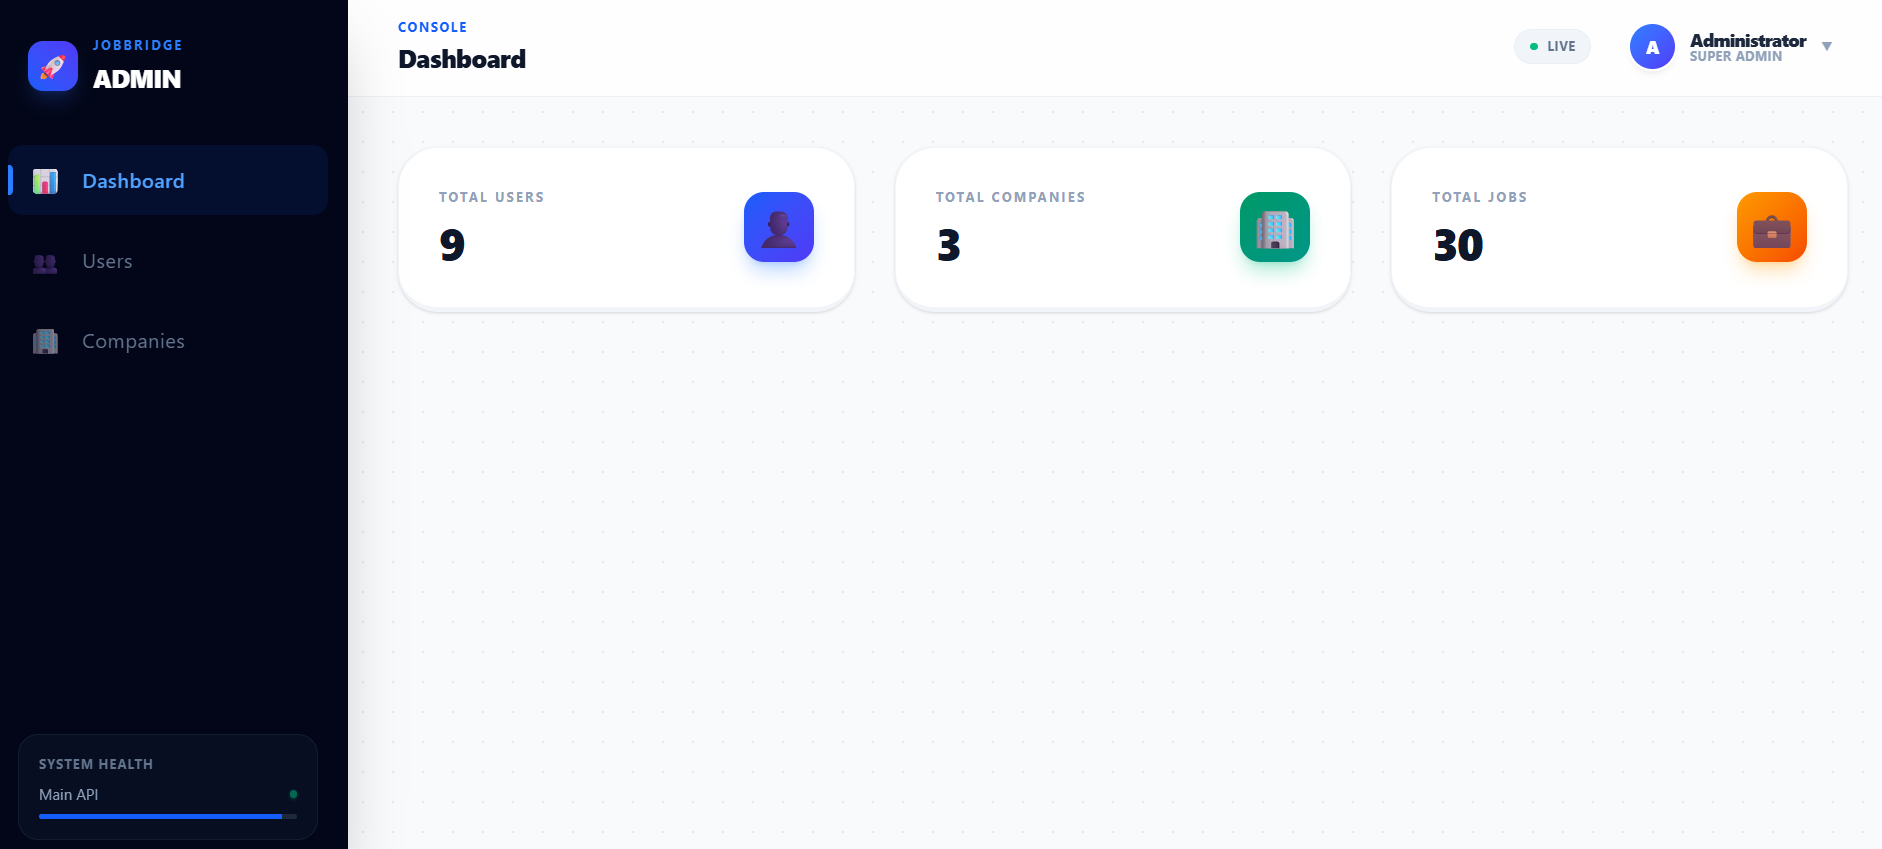
\includegraphics[width=1.15\textwidth]{so-do-chuong-4/screens/màn hình dashboard dành cho admin.png}%
    }
    \caption{Giao diện dashboard dành cho quản trị viên}
    \label{fig:ui-admin}
\end{figure}

\section{Triển khai tự động bằng CI/CD và GitOps}
\label{sec:trien-khai-cicd}
\label{sec:trien-khai}

Hệ thống được triển khai theo quy trình CI/CD tự động kết hợp GitOps. Khi mã nguồn được đưa lên nhánh chính, GitHub Actions kích hoạt pipeline để kiểm tra mã nguồn, build image cho các service, quét lỗ hổng bảo mật và đẩy image lên Azure Container Registry. Sau đó, pipeline triển khai cập nhật phiên bản image trong cấu hình Helm dùng cho môi trường production.

Argo CD chạy trong cụm AKS theo dõi repository cấu hình triển khai. Khi phát hiện tag image mới, Argo CD tự động đồng bộ trạng thái mong muốn từ Git vào cluster theo cơ chế rolling update.

Trong lần quan sát ở Hình \ref{fig:argocd-live}, giao diện Argo CD ghi nhận ứng dụng ở trạng thái khỏe mạnh, đã đồng bộ và lần đồng bộ gần nhất hoàn tất sau khoảng một phút. Điều này cho thấy quy trình phát hành không cần thao tác thủ công trực tiếp trên cluster.

\begin{figure}[H]
    \centering
    \makebox[\textwidth][c]{%
        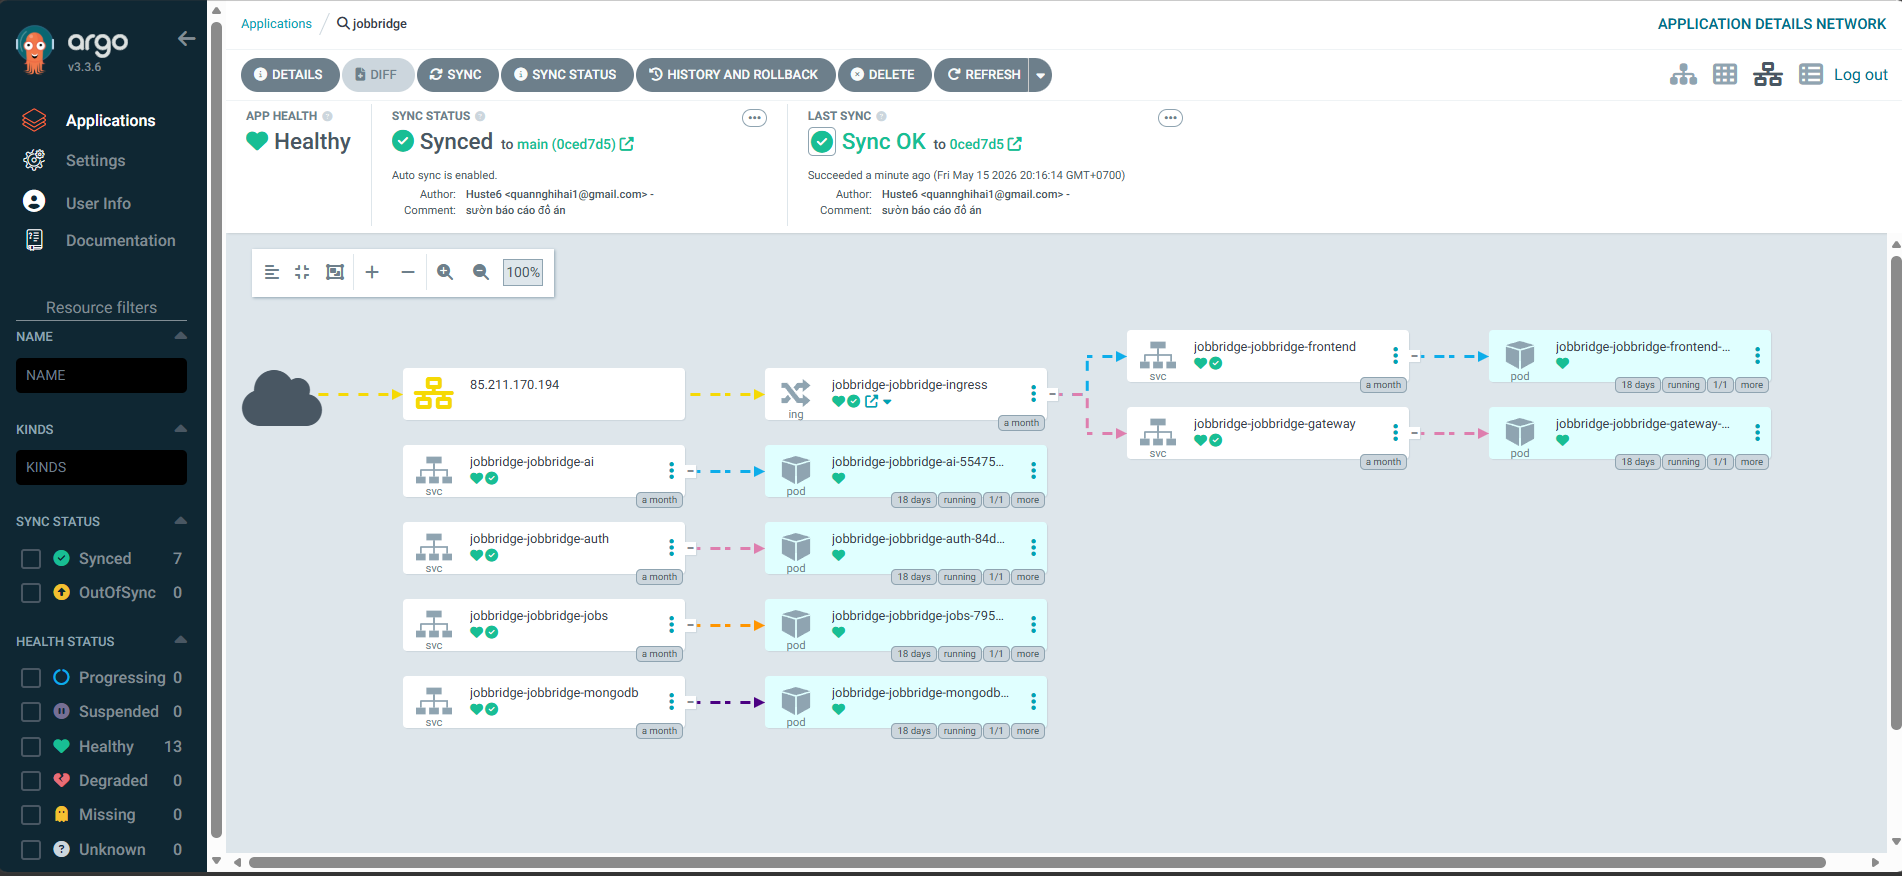
\includegraphics[width=1.15\textwidth]{so-do-chuong-4/screens/argocd_live.png}%
    }
    \caption{Trạng thái đồng bộ GitOps của ứng dụng trên Argo CD}
    \label{fig:argocd-live}
\end{figure}

So với triển khai thủ công, quy trình này tối ưu ở ba điểm. Thứ nhất, thời gian phát hành ngắn hơn vì quá trình build, gắn tag image và cập nhật cấu hình triển khai được tự động hóa. Thứ hai, khả năng truy vết tốt hơn vì mỗi phiên bản chạy trên cluster gắn với một commit cụ thể. Thứ ba, rủi ro sai khác môi trường giảm xuống vì trạng thái triển khai được khai báo trong Git và Argo CD liên tục so sánh với trạng thái thực tế của cluster.

\section{Đánh giá khả năng vận hành và mở rộng}
\label{sec:danh-gia-van-hanh}

\subsection{Cấu hình tài nguyên triển khai}

Để hệ thống có khả năng phản ứng trước tải biến thiên, các service quan trọng được cấu hình Horizontal Pod Autoscaler. Bảng \ref{tab:k8s-hpa} trình bày cấu hình HPA và Pod Disruption Budget đang áp dụng trên môi trường AKS.

\begin{table}[H]
\centering
\caption{Cấu hình HPA và PDB của các service trên AKS}
\label{tab:k8s-hpa}
\small
\begin{tabular}{|p{3cm}|p{2.1cm}|p{2.1cm}|p{2.4cm}|p{2.5cm}|}
\hline
\textbf{Service} & \textbf{Replica tối thiểu} & \textbf{Replica tối đa} & \textbf{Ngưỡng CPU} & \textbf{Pod tối thiểu sẵn sàng} \\ \hline
Frontend & 1 & 3 & 75\% & 1 \\ \hline
Gateway & 1 & 5 & 70\% & 1 \\ \hline
Auth Service & 1 & 5 & 70\% & 1 \\ \hline
Jobs Service & 1 & 5 & 70\% & 1 \\ \hline
AI Service & 1 & 3 & 75\% & 1 \\ \hline
\end{tabular}
\end{table}

Với cấu hình trên, hệ thống có thể tự động tăng số lượng replica khi CPU vượt ngưỡng. Đây là cơ sở để đáp ứng yêu cầu phi chức năng về khả năng phục vụ nhiều người dùng đồng thời, thay vì cố định mỗi service ở một Pod duy nhất.

\subsection{Giám sát hệ thống}

Hệ thống sử dụng Prometheus và Grafana để thu thập, lưu trữ và trực quan hóa metric vận hành. Prometheus lấy dữ liệu từ các Pod và ingress, còn Grafana cung cấp dashboard theo dõi tình trạng API, Pod và tài nguyên. Việc có hệ thống giám sát giúp quá trình đánh giá không chỉ dựa trên cảm nhận giao diện mà dựa trên các chỉ số như tỷ lệ lỗi, lưu lượng request, độ trễ và mức sử dụng CPU/memory.

Hình \ref{fig:grafana-live} minh họa dashboard theo dõi sức khỏe API và Pod. Dashboard này cho phép quan sát tỷ lệ Pod sẵn sàng, tỷ lệ lỗi HTTP, lưu lượng request đi qua ingress, độ trễ request và lưu lượng mạng theo Pod. Khi triển khai thực tế, các chỉ số này giúp phát hiện sớm lỗi 5xx, service chậm hoặc Pod hoạt động bất thường.

\begin{figure}[H]
    \centering
    \makebox[\textwidth][c]{%
        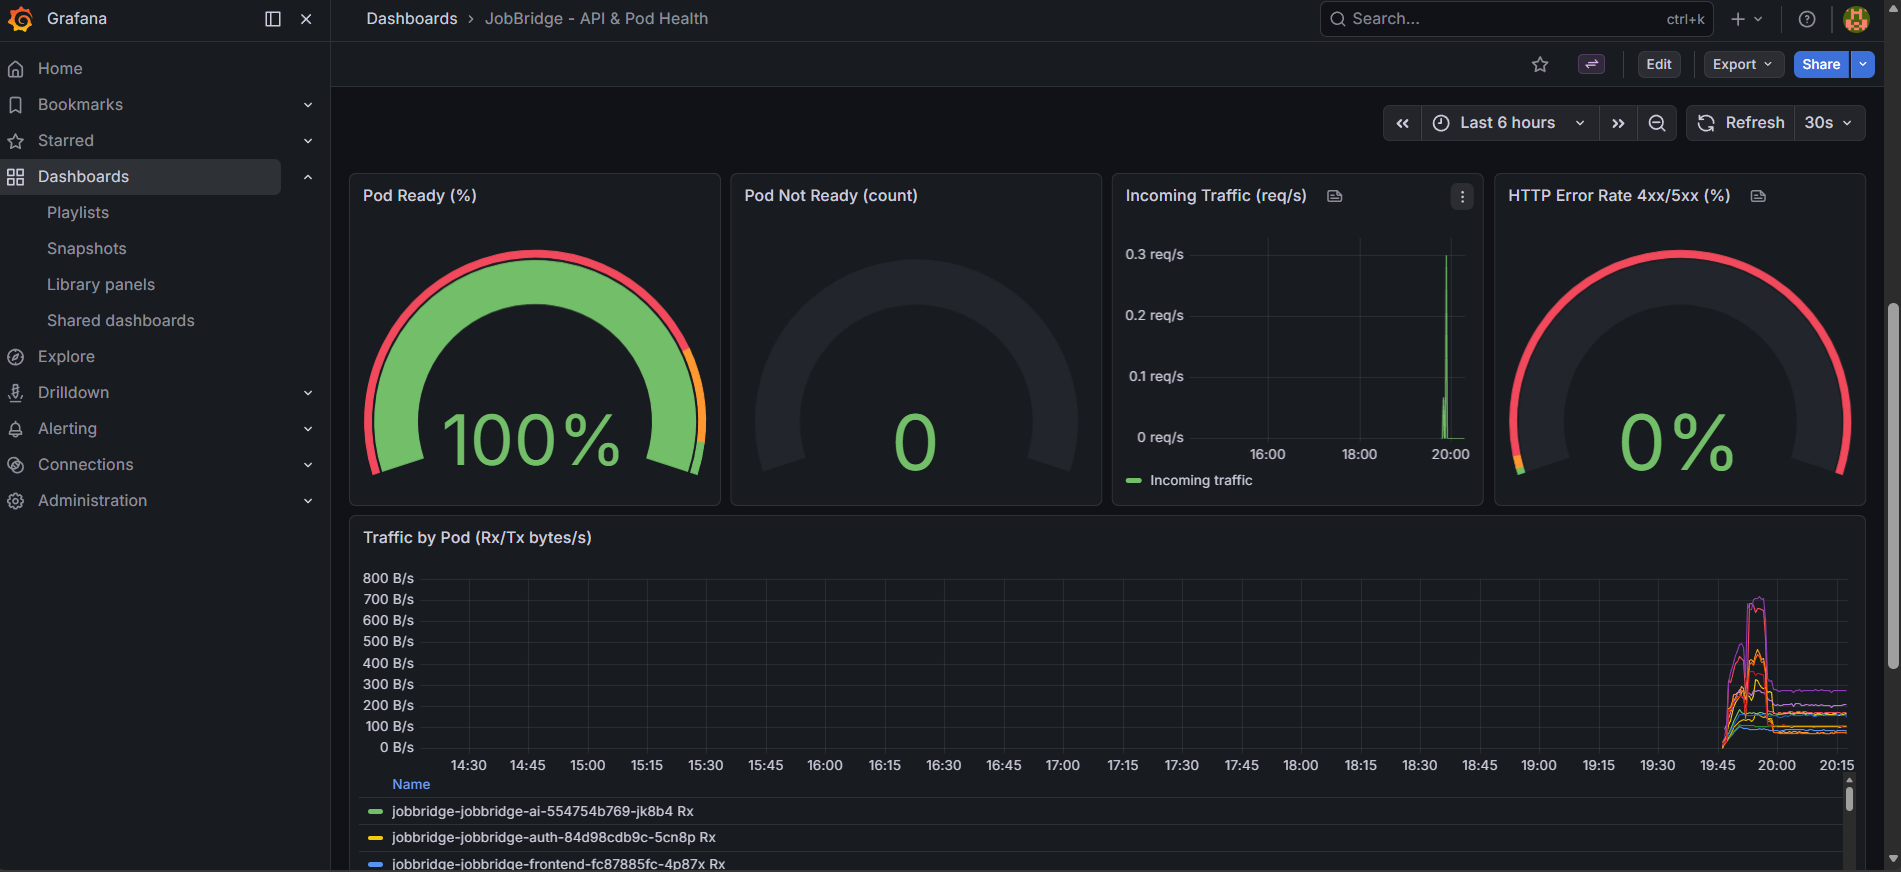
\includegraphics[width=1.15\textwidth]{so-do-chuong-4/screens/grafana_live.png}%
    }
    \caption{Dashboard Grafana giám sát sức khỏe API và Pod}
    \label{fig:grafana-live}
\end{figure}

Hình \ref{fig:grafana-stress} minh họa dashboard dùng trong quá trình thử tải. Dashboard này tập trung vào mức sử dụng CPU, memory, network và số lần restart của Pod. Các panel này giúp xác định service nào trở thành điểm nghẽn khi tải tăng, đồng thời kiểm chứng cơ chế tự động mở rộng có kích hoạt đúng ngưỡng hay không.

\begin{figure}[H]
    \centering
    \makebox[\textwidth][c]{%
        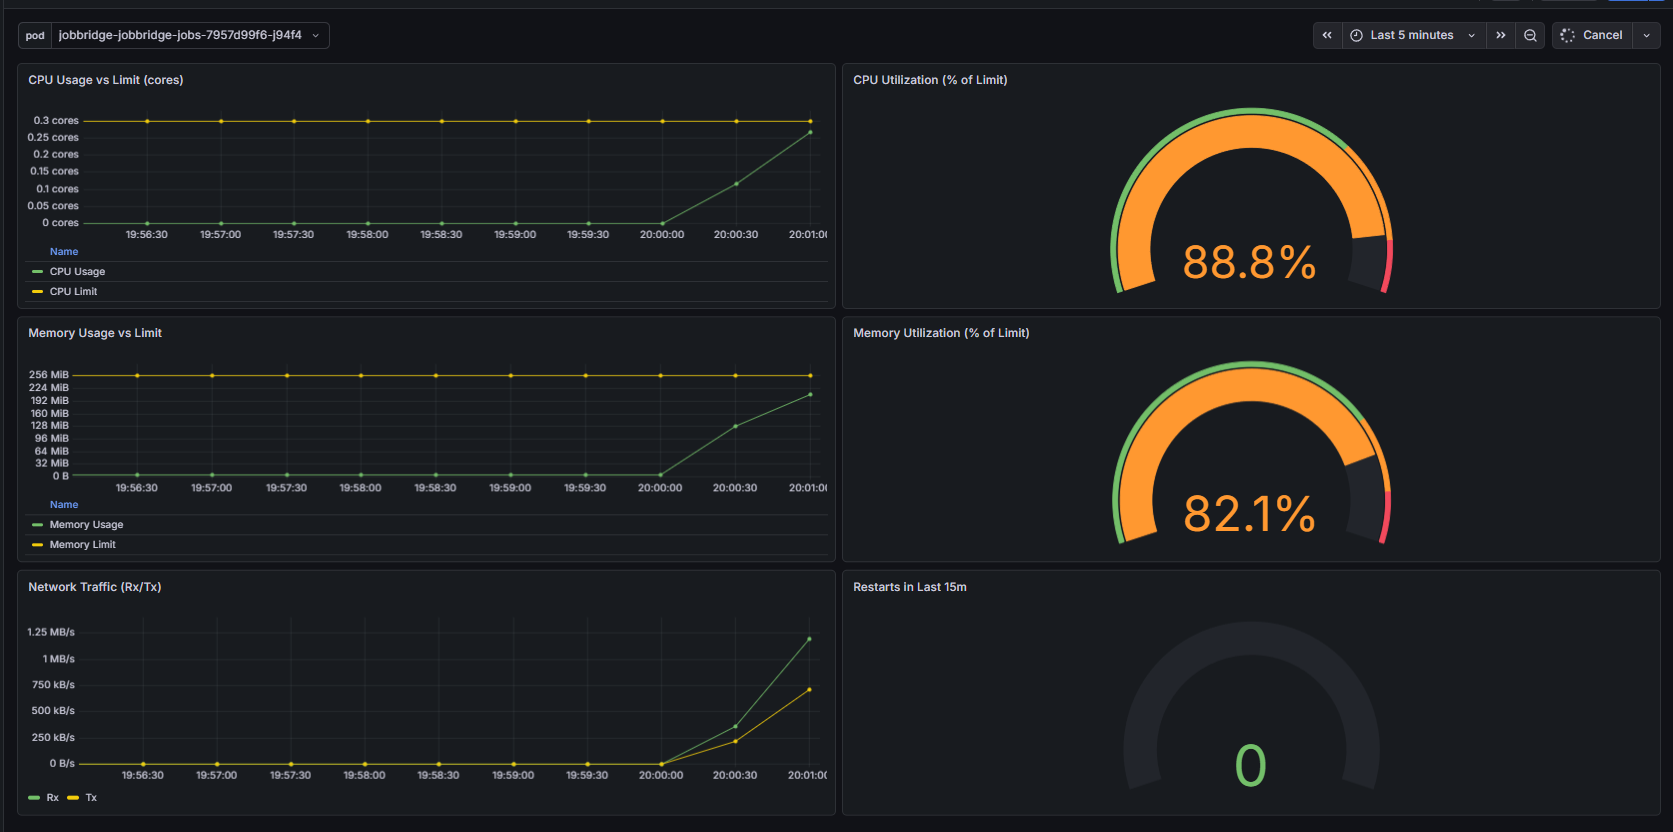
\includegraphics[width=1.15\textwidth]{so-do-chuong-4/screens/grafana_stress_test.png}%
    }
    \caption{Dashboard Grafana theo dõi tài nguyên trong quá trình thử tải}
    \label{fig:grafana-stress}
\end{figure}

\subsection{Kịch bản thực nghiệm tải}

Mục đích của thực nghiệm tải là kiểm chứng khả năng xử lý request đồng thời và phản ứng tự động của HPA khi service chịu áp lực. Kịch bản được thực hiện bằng k6 trong cluster, tập trung vào API danh sách việc làm. Đây là nhóm API phù hợp để thử nghiệm vì request đi qua Gateway, đến Jobs Service và truy vấn MongoDB, tạo tải thực tế lên cả tầng định tuyến lẫn tầng nghiệp vụ.

Kịch bản tải tăng dần lên 1.500 virtual users trong 30 giây, tiếp tục tăng và duy trì ở mức 3.000 virtual users trong 2 phút, sau đó giảm dần về 0. Trong quá trình thử nghiệm, các chỉ số CPU, số lượng replica, tỷ lệ lỗi và trạng thái Pod được quan sát qua Grafana và Kubernetes metrics.

\begin{table}[H]
\centering
\caption{Mục tiêu và kết quả quan sát của thực nghiệm tải}
\label{tab:load-test-result}
\begin{tabular}{|p{0.34\textwidth}|p{0.5\textwidth}|}
\hline
\textbf{Nội dung đánh giá} & \textbf{Kết quả quan sát} \\ \hline
Nghiệp vụ thử nghiệm & API danh sách việc làm, đi qua Gateway và Jobs Service. \\ \hline
Mức tải cao nhất & 3.000 virtual users trong giai đoạn duy trì tải. \\ \hline
Service chịu tải chính & Gateway và Jobs Service. \\ \hline
Phản ứng autoscaling & Jobs Service tăng từ 1 lên 4 Pod; Gateway tăng từ 1 lên 2 Pod khi CPU vượt ngưỡng. \\ \hline
Mức CPU quan sát được & Jobs Service đạt khoảng 222\% so với ngưỡng 70\%; Gateway đạt khoảng 130\% so với ngưỡng 70\%. \\ \hline
Tỷ lệ lỗi kết nối & Không ghi nhận lỗi kết nối hoặc timeout trong lần quan sát. \\ \hline
\end{tabular}
\end{table}

Kết quả trên cho thấy hệ thống đã được tối ưu ở mức vận hành cơ bản: khi tải tăng, Gateway và Jobs Service không giữ nguyên một replica mà tự động mở rộng để chia tải. Điều này tốt hơn triển khai tĩnh vì giúp tài nguyên được dùng linh hoạt: lúc tải thấp hệ thống tiết kiệm chi phí bằng số Pod tối thiểu, lúc tải cao hệ thống tự tăng replica để duy trì khả năng phục vụ.

Tuy nhiên, kết quả này chưa đồng nghĩa với việc hệ thống đã sẵn sàng cho quy mô một triệu người dùng đồng thời. Môi trường thực nghiệm hiện tại sử dụng cấu hình tiết kiệm chi phí, trong đó số node AKS và số replica tối đa còn giới hạn.

Để tiến tới quy mô rất lớn, hệ thống cần mở rộng thêm node pool, tăng giới hạn HPA, tối ưu cache cho dữ liệu đọc nhiều, bổ sung rate limiting, tách MongoDB sang cụm managed có replica/sharding và đưa các tác vụ AI tốn thời gian vào hàng đợi bất đồng bộ.

\section{Đánh giá mức độ đáp ứng yêu cầu phi chức năng}

\subsection{Tự động hóa triển khai}

Về tự động hóa triển khai, hệ thống đã đáp ứng mục tiêu phát hành tự động: commit mới trên nhánh chính có thể kích hoạt CI/CD, cập nhật image và để Argo CD đồng bộ lên môi trường production. Lợi ích chính là giảm thao tác thủ công, tăng khả năng rollback và giúp phiên bản triển khai luôn có dấu vết trong Git.

\begin{figure}[H]
    \centering
    \makebox[\textwidth][c]{%
        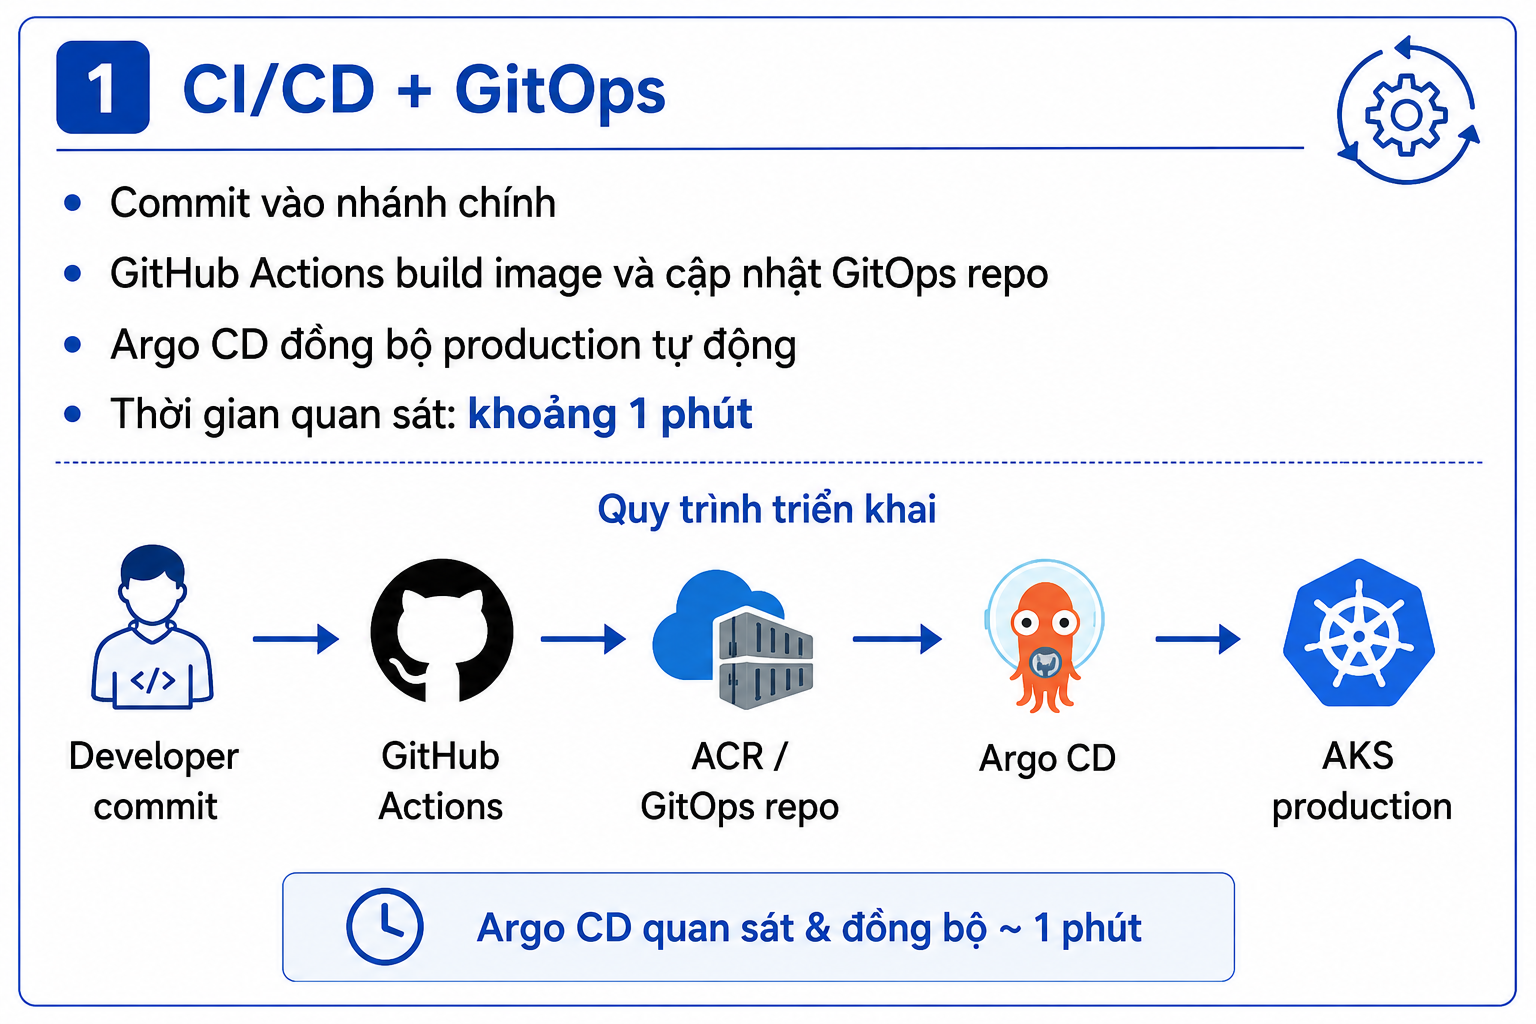
\includegraphics[width=1.15\textwidth]{so-do-chuong-4/evaluation/cicd_gitops.png}%
    }
    \caption{Đánh giá phi chức năng về tự động hóa triển khai CI/CD và GitOps}
    \label{fig:nfr-cicd-gitops}
\end{figure}

\subsection{Khả năng mở rộng}

Về khả năng mở rộng, hệ thống đã chứng minh được khả năng scale ngang ở cấp Pod trong kịch bản tải cao. Việc Jobs Service và Gateway tự tăng replica cho thấy kiến trúc triển khai không bị khóa vào một instance đơn lẻ. Đây là tiền đề quan trọng để mở rộng lên mức 1.000 người dùng đồng thời và cao hơn khi bổ sung thêm tài nguyên node.

\begin{figure}[H]
    \centering
    \makebox[\textwidth][c]{%
        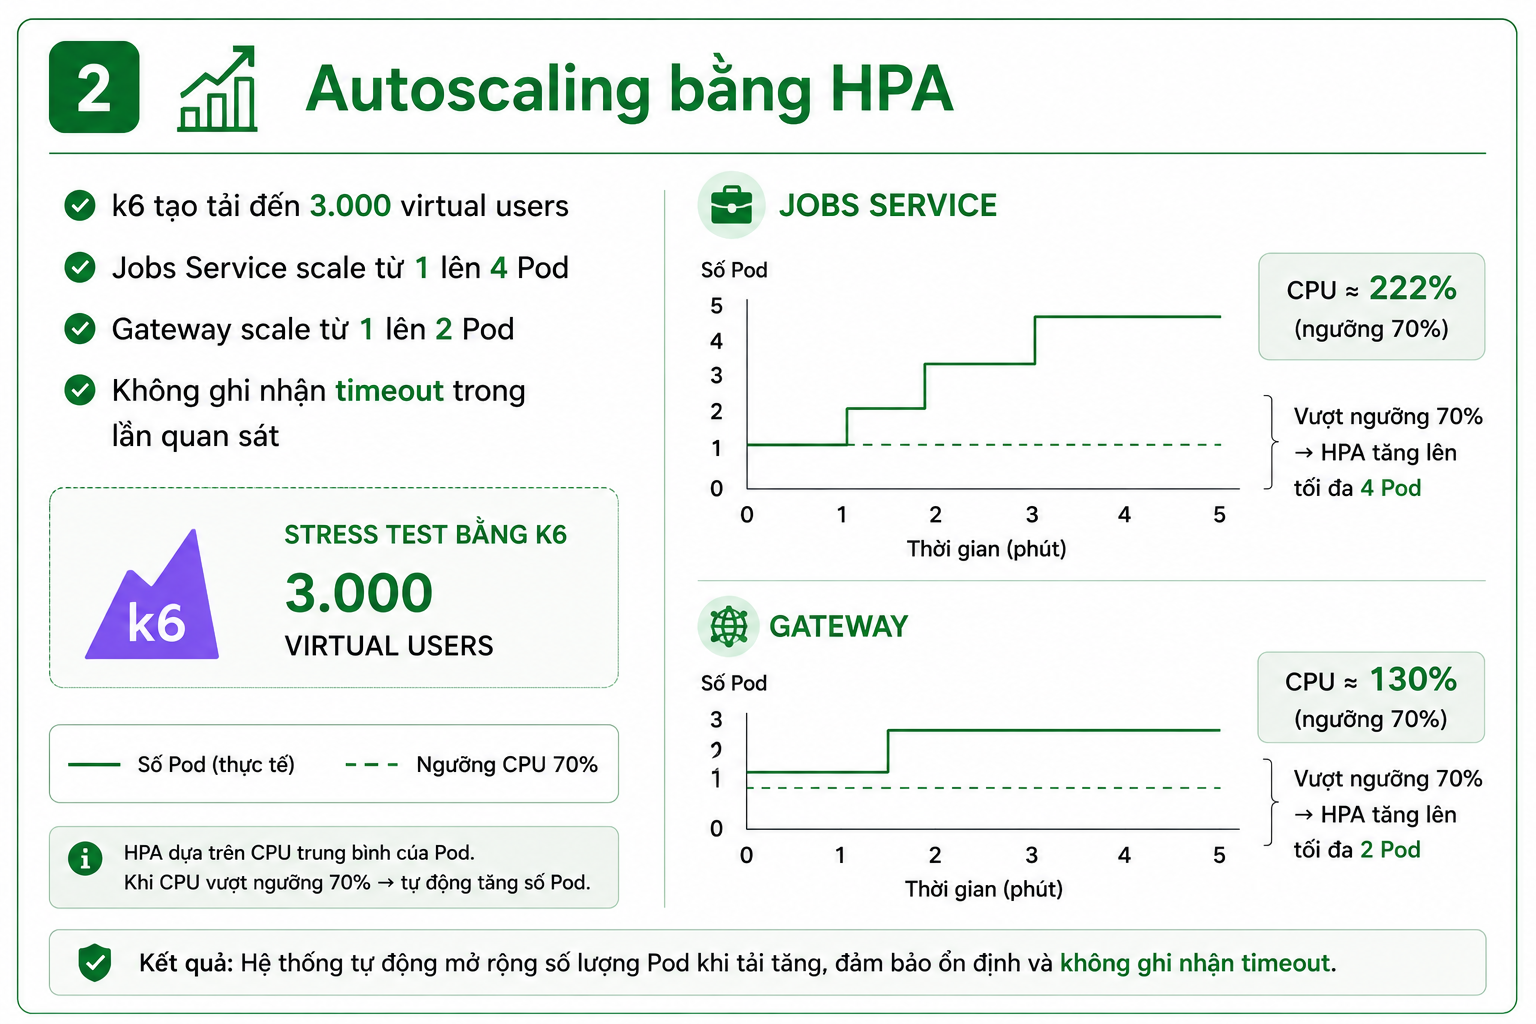
\includegraphics[width=1.15\textwidth]{so-do-chuong-4/evaluation/autoscalling.png}%
    }
    \caption{Đánh giá phi chức năng về khả năng mở rộng bằng Horizontal Pod Autoscaler}
    \label{fig:nfr-autoscaling}
\end{figure}

\subsection{Khả năng quan sát}

Về khả năng quan sát, Prometheus và Grafana cung cấp các chỉ số cần thiết để đánh giá vận hành thay vì chỉ dựa vào trạng thái ``chạy được''. Các dashboard hiện tại cho phép theo dõi lỗi HTTP, độ trễ, lưu lượng request, CPU, memory, network và số lần restart Pod. Khi có thêm dữ liệu thử tải ở các phiên bản tiếp theo, các biểu đồ này có thể được dùng để trình bày rõ hơn độ trễ ở các phân vị cao và tỷ lệ lỗi trong báo cáo in.

\begin{figure}[H]
    \centering
    \makebox[\textwidth][c]{%
        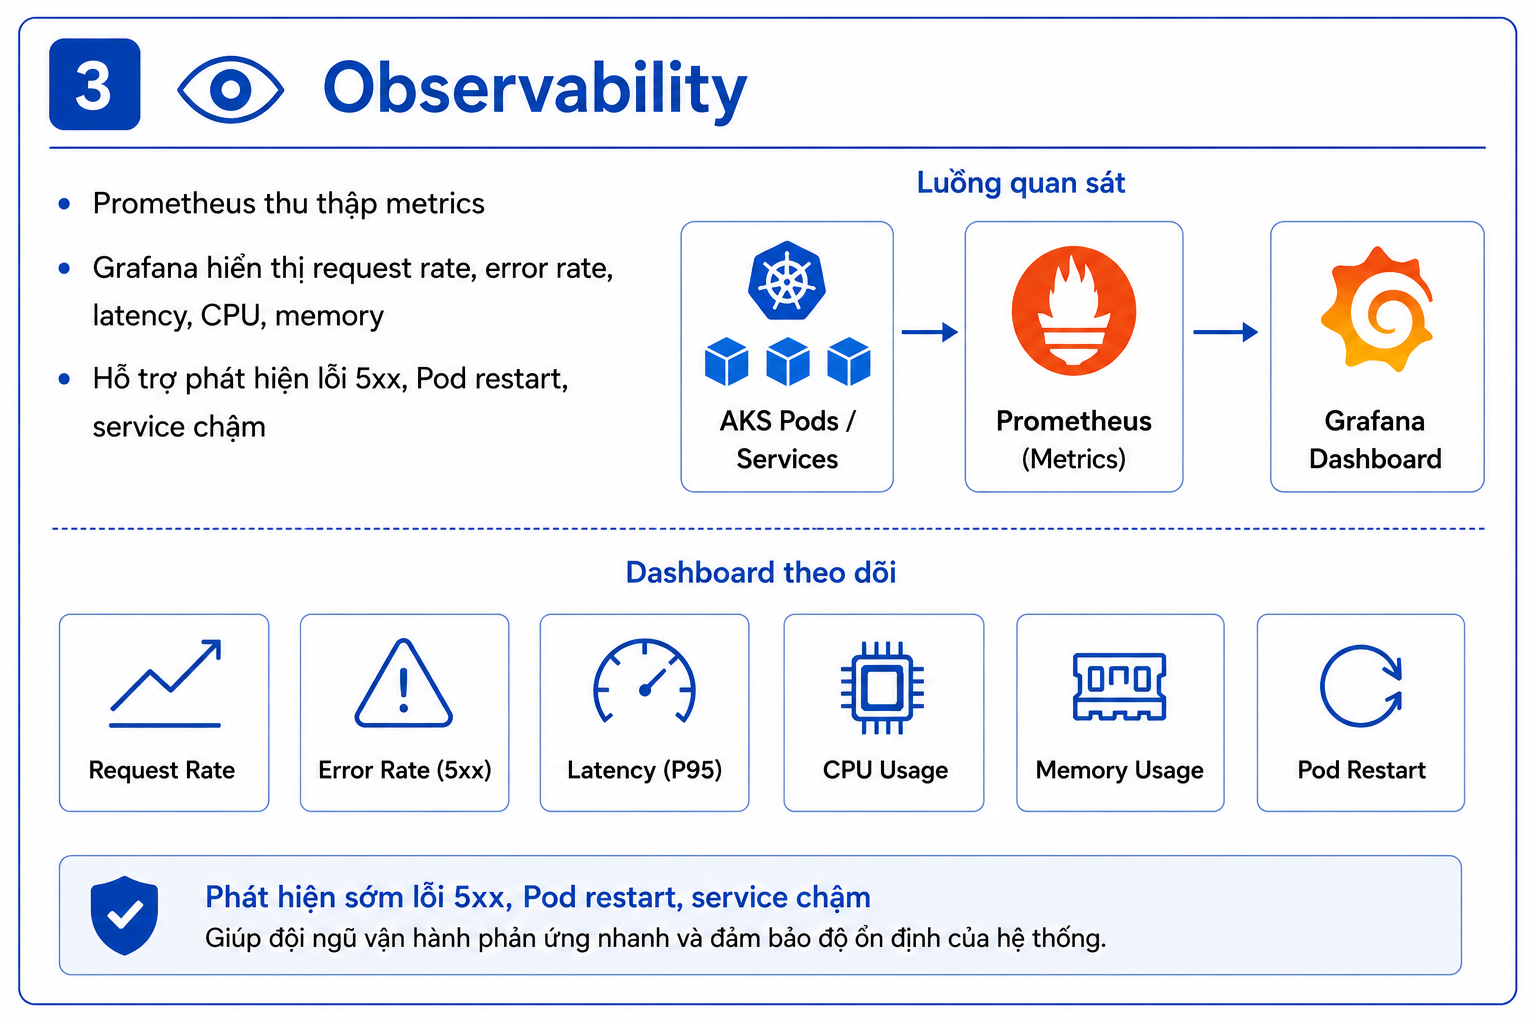
\includegraphics[width=1.15\textwidth]{so-do-chuong-4/evaluation/observ.png}%
    }
    \caption{Đánh giá phi chức năng về khả năng quan sát hệ thống bằng Prometheus và Grafana}
    \label{fig:nfr-observability}
\end{figure}

\subsection{Giới hạn và hướng tối ưu tiếp theo}

Về giới hạn, các chức năng AI phụ thuộc vào thời gian phản hồi của LLM API bên ngoài nên không thể đánh giá giống các API đọc dữ liệu thông thường. Với nhóm API AI, hướng tối ưu tiếp theo là giới hạn tần suất gọi, cache ngữ cảnh đã xử lý, đưa tác vụ dài vào queue và tách riêng autoscaling cho AI Service dựa trên số request hoặc hàng đợi thay vì chỉ dựa trên CPU.

\begin{figure}[H]
    \centering
    \makebox[\textwidth][c]{%
        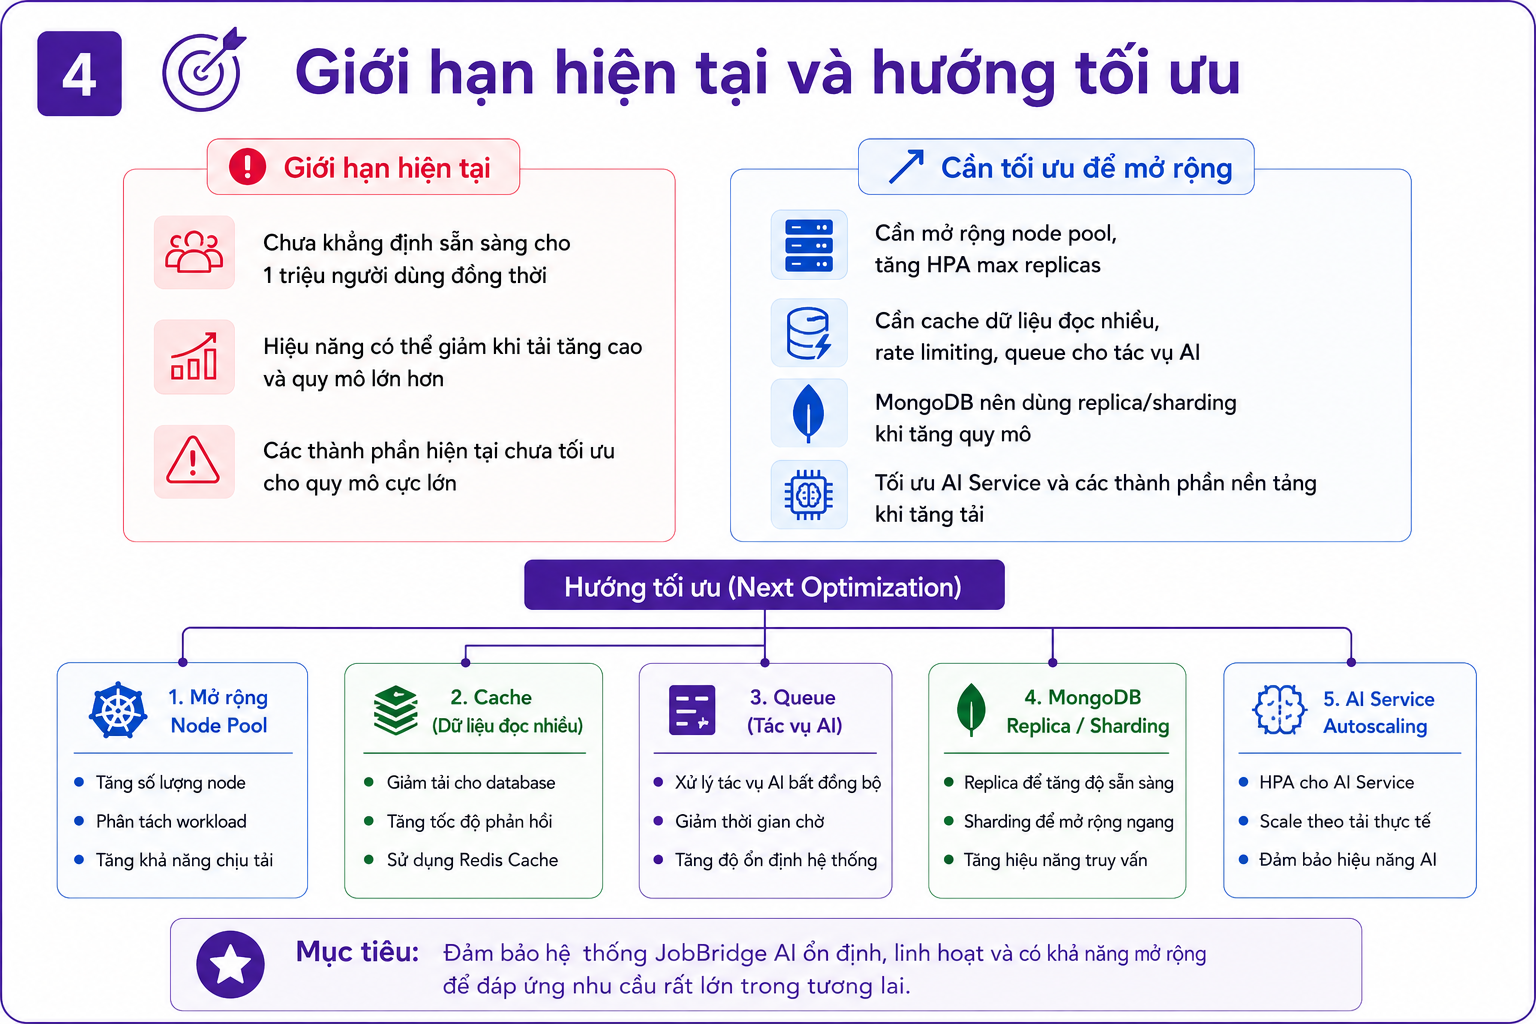
\includegraphics[width=1.15\textwidth]{so-do-chuong-4/evaluation/gioi_han_huong_toi_uu.png}%
    }
    \caption{Giới hạn hiện tại và định hướng tối ưu khi mở rộng hệ thống}
    \label{fig:nfr-limit-optimization}
\end{figure}

\section{Kết chương}

Chương này đã trình bày kết quả triển khai hệ thống JobBridge AI trên môi trường AKS, mô tả các giao diện chức năng chính, phân tích quy trình CI/CD GitOps và đánh giá khả năng vận hành thông qua giám sát cùng thực nghiệm tải. Kết quả cho thấy hệ thống không chỉ hiện thực được các chức năng nghiệp vụ chính mà còn có khả năng phát hành tự động, quan sát trạng thái vận hành và tự động mở rộng một số service khi tải tăng.

Các kết quả thực nghiệm cũng chỉ ra giới hạn cần tiếp tục tối ưu nếu hướng tới quy mô rất lớn, đặc biệt là mở rộng node pool, tối ưu cơ sở dữ liệu, cache dữ liệu đọc nhiều và xử lý bất đồng bộ cho các tác vụ AI. Những nội dung này là cơ sở để Chương 5 phân tích sâu hơn các giải pháp kỹ thuật và đóng góp nổi bật của đồ án.

\end{document}
